\documentclass{article}
\usepackage[utf8]{inputenc}
\usepackage{graphicx}
\usepackage{geometry}
\usepackage{listings}
\usepackage{hyperref}

\geometry{
 a4paper,
 total={170mm,257mm},
 left=20mm,
 top=20mm,
}

\title{Práctica 5: Aplicación de Gestión de Tareas con Navegación y Carga Diferida}
\author{Kirbi Xavier Huerta Salinas}
\date{Octubre 2025}

\begin{document}

\maketitle

\section{Introducción}
El presente documento detalla el desarrollo de una aplicación móvil para la gestión de tareas, construida con Ionic y Angular. El objetivo de la práctica es aplicar conceptos clave de desarrollo de aplicaciones móviles, como la creación de componentes, navegación, persistencia de datos y optimización de carga.

La aplicación permite a los usuarios crear, visualizar, editar y eliminar tareas, las cuales se almacenan localmente en el dispositivo para garantizar la persistencia de la información entre sesiones.

\section{Cumplimiento de Requisitos}
La aplicación implementa todos los requisitos solicitados en el documento de la práctica:
\begin{itemize}
    \item \textbf{Creación de Páginas:} Se crearon tres páginas principales: \texttt{Home} (para listar tareas), \texttt{Tarea} (para crear una nueva tarea) y \texttt{TareaDetalles} (para editar una tarea existente).
    \item \textbf{Navegación:} Se configuró un sistema de rutas en Angular para navegar entre las páginas mencionadas.
    \item \textbf{Lazy Loading:} Todas las rutas de las páginas se implementaron con carga diferida (lazy loading) utilizando la función \texttt{loadComponent} para optimizar el rendimiento inicial de la aplicación.
    \item \textbf{Servicio y Persistencia:} Se desarrolló un servicio (\texttt{TareaService}) que centraliza la lógica de negocio (CRUD) y utiliza el \texttt{localStorage} del navegador para guardar y recuperar las tareas.
    \item \textbf{Diseño de UI:} La interfaz es sencilla y funcional, utilizando los componentes de Ionic para una experiencia de usuario nativa.
    \item \textbf{Validaciones:} El formulario de creación y edición de tareas incluye validaciones para campos requeridos y para asegurar que la fecha de vencimiento sea siempre una fecha futura.
\end{itemize}

\section{Estructura y Organización del Proyecto}
El proyecto sigue la estructura estándar de una aplicación de Angular, con los componentes de la aplicación ubicados en la carpeta \texttt{src/app}. Las páginas, servicios y modelos de datos se organizaron en sus respectivas carpetas para mantener el código ordenado y mantenible.

\begin{itemize}
    \item \texttt{src/app/pages/}: Contiene los componentes de página (\texttt{TareaPage}, \texttt{TareaDetallesPage}).
    \item \texttt{src/app/services/}: Contiene el servicio de lógica de negocio (\texttt{TareaService}).
    \item \texttt{src/app/models/}: Define la interfaz del modelo de datos (\texttt{Tarea}).
    \item \texttt{src/app/validators/}: Contiene validadores de formularios personalizados.
\end{itemize}

\section{Detalles de Implementación}

\subsection{Uso de Lazy Loading}
La carga diferida se configuró en \texttt{src/app/app.routes.ts}. Cada ruta utiliza \texttt{loadComponent} para cargar los componentes de página solo cuando son necesarios.

\begin{lstlisting}[breaklines=true]
import { Routes } from '@angular/router';

export const routes: Routes = [
  {
    path: 'home',
    loadComponent: () => import('./home/home.page').then((m) => m.HomePage),
  },
  {
    path: 'tarea',
    loadComponent: () => import('./pages/tarea/tarea.page').then( m => m.TareaPage)
  },
  {
    path: 'tarea-detalles/:id',
    loadComponent: () => import('./pages/tarea-detalles/tarea-detalles.page').then( m => m.TareaDetallesPage)
  },
];
\end{lstlisting}

\subsection{Persistencia con LocalStorage}
El servicio \texttt{TareaService} es responsable de interactuar con \texttt{localStorage} para persistir los datos. Los métodos \texttt{saveTareas} y \texttt{getTareas} se encargan de la serialización y deserialización de los datos de las tareas.

\begin{lstlisting}[breaklines=true]
@Injectable({
  providedIn: 'root'
})
export class TareaService {
  private readonly storageKey = 'tareas';

  getTareas(): Tarea[] {
    const tareasJson = localStorage.getItem(this.storageKey);
    if (tareasJson) {
      return JSON.parse(tareasJson).map((tarea: any) => ({
        ...tarea,
        fechaVencimiento: new Date(tarea.fechaVencimiento)
      }));
    }
    return [];
  }

  private saveTareas(tareas: Tarea[]): void {
    localStorage.setItem(this.storageKey, JSON.stringify(tareas));
  }
  // ... otros metodos CRUD
}
\end{lstlisting}

\subsection{Validaciones de Formulario}
Se utilizó un validador personalizado (\texttt{fechaFuturaValidator}) para el campo de fecha, asegurando que el usuario no pueda seleccionar una fecha que ya ha pasado. Este validador se combina con los validadores estándar de Angular para campos requeridos.

\begin{lstlisting}[breaklines=true]
// En el componente TareaPage o TareaDetallesPage
this.tareaForm = this.fb.group({
  titulo: ['', Validators.required],
  descripcion: ['', Validators.required],
  fechaVencimiento: [null, [Validators.required, fechaFuturaValidator]]
});

// Mensaje de error en el HTML
<div *ngIf="tareaForm.get('fechaVencimiento')?.hasError('fechaPasada')">
  La fecha debe ser futura.
</div>
\end{lstlisting}




\section{Compilación para Android con Capacitor}
Para empaquetar la aplicación para Android, se utilizó Capacitor. Este proceso convierte la aplicación web en un proyecto nativo de Android que puede ser gestionado con Android Studio.

Los pasos seguidos fueron los siguientes:
\begin{enumerate}
    \item \textbf{Instalar dependencias de Capacitor:}
    \begin{verbatim}
npm install @capacitor/core @capacitor/cli
    \end{verbatim}

    \item \textbf{Inicializar Capacitor:} Se crea el archivo de configuración principal.
    \begin{verbatim}
npx cap init
    \end{verbatim}

    \item \textbf{Construir la aplicación web:} Se generan los archivos estáticos del proyecto de Angular.
    \begin{verbatim}
npm run build
    \end{verbatim}

    \item \textbf{Añadir la plataforma Android:} Se crea el proyecto nativo de Android.
    \begin{verbatim}
npx cap add android
    \end{verbatim}

    \item \textbf{Sincronizar los recursos web:} Se copian los archivos web al proyecto nativo.
    \begin{verbatim}
npx cap sync
    \end{verbatim}

    \item \textbf{Abrir en Android Studio:} Finalmente, se abre el proyecto en el IDE de Android para compilar y ejecutar.
    \begin{verbatim}
npx cap open android
    \end{verbatim}
\end{enumerate}



\section{Demostración en Video}
Se grabó un video que muestra la aplicación funcionando en un dispositivo móvil Android. El video demuestra la creación, edición, y eliminación de tareas, así como la correcta funcionalidad de las validaciones y la persistencia de datos.

El video se puede visualizar en el siguiente enlace:
\href{https://correobuap-my.sharepoint.com/:v:/g/personal/kirbi_huertas_alumno_buap_mx/ERhO-CAdlztNmy3Wuwh2q4IB6dL--OChuUR7Iv7fA9dB9Q?nav=eyJyZWZlcnJhbEluZm8iOnsicmVmZXJyYWxBcHAiOiJPbmVEcml2ZUZvckJ1c2luZXNzIiwicmVmZXJyYWxBcHBQbGF0Zm9ybSI6IldlYiIsInJlZmVycmFsTW9kZSI6InZpZXciLCJyZWZlcnJhbFZpZXciOiJNeUZpbGVzTGlua0NvcHkifX0&e=i78Fpx}{Ver video de la aplicación en funcionamiento}

\section{Repositorio}
El código fuente de este proyecto se encuentra disponible en el siguiente repositorio de GitHub:
\url{https://github.com/XavierHuerta/admin-tasks.git}


\section{Capturas de Pantalla}

\begin{figure}[htbp]
\centering
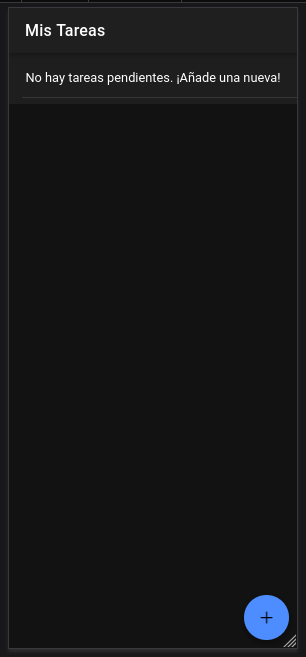
\includegraphics[width=0.4\textwidth]{captura_home.png}
\caption{Página principal con la lista de tareas.}
\end{figure}

\begin{figure}[htbp]
\centering
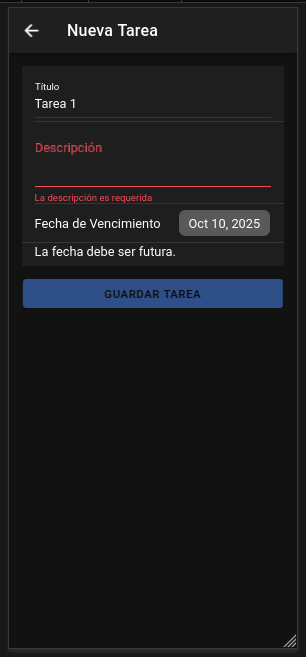
\includegraphics[width=0.4\textwidth]{captura_crear.png}
\caption{Formulario de creación de una nueva tarea.}
\end{figure}

\begin{figure}[htbp]
\centering
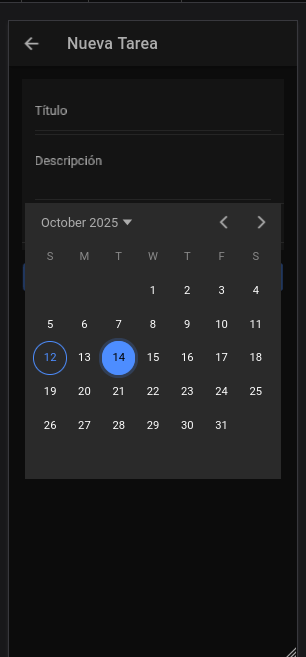
\includegraphics[width=0.4\textwidth]{captura_fecha.png}
\caption{ion-datetime para seleccionar la fecha de vencimiento.}
\end{figure}

\begin{figure}[htbp]
\centering
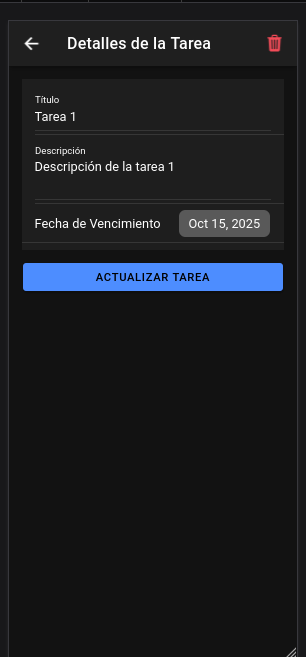
\includegraphics[width=0.4\textwidth]{captura_detalles.png}
\caption{Formulario de edición de una tarea existente.}
\end{figure}

\begin{figure}[htbp]
\centering
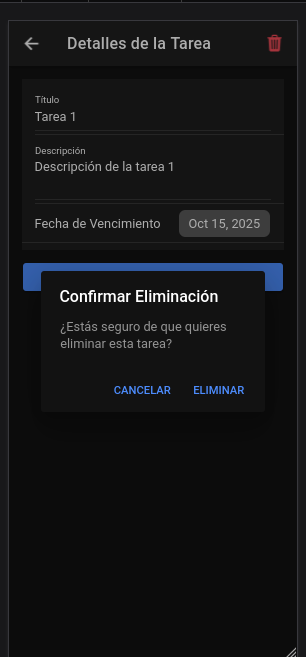
\includegraphics[width=0.4\textwidth]{captura_eliminar.png}
\caption{Mensaje al querer eliminar una tarea.}
\end{figure}

\end{document}
